\documentclass[]{article}
\usepackage{lmodern}
\usepackage{amssymb,amsmath}
\usepackage{ifxetex,ifluatex}
\usepackage{fixltx2e} % provides \textsubscript
\ifnum 0\ifxetex 1\fi\ifluatex 1\fi=0 % if pdftex
  \usepackage[T1]{fontenc}
  \usepackage[utf8]{inputenc}
\else % if luatex or xelatex
  \ifxetex
    \usepackage{mathspec}
  \else
    \usepackage{fontspec}
  \fi
  \defaultfontfeatures{Ligatures=TeX,Scale=MatchLowercase}
\fi
% use upquote if available, for straight quotes in verbatim environments
\IfFileExists{upquote.sty}{\usepackage{upquote}}{}
% use microtype if available
\IfFileExists{microtype.sty}{%
\usepackage{microtype}
\UseMicrotypeSet[protrusion]{basicmath} % disable protrusion for tt fonts
}{}
\usepackage[margin=1in]{geometry}
\usepackage{hyperref}
\hypersetup{unicode=true,
            pdftitle={seasadj simu},
            pdfauthor={linyiguo},
            pdfborder={0 0 0},
            breaklinks=true}
\urlstyle{same}  % don't use monospace font for urls
\usepackage{color}
\usepackage{fancyvrb}
\newcommand{\VerbBar}{|}
\newcommand{\VERB}{\Verb[commandchars=\\\{\}]}
\DefineVerbatimEnvironment{Highlighting}{Verbatim}{commandchars=\\\{\}}
% Add ',fontsize=\small' for more characters per line
\usepackage{framed}
\definecolor{shadecolor}{RGB}{248,248,248}
\newenvironment{Shaded}{\begin{snugshade}}{\end{snugshade}}
\newcommand{\AlertTok}[1]{\textcolor[rgb]{0.94,0.16,0.16}{#1}}
\newcommand{\AnnotationTok}[1]{\textcolor[rgb]{0.56,0.35,0.01}{\textbf{\textit{#1}}}}
\newcommand{\AttributeTok}[1]{\textcolor[rgb]{0.77,0.63,0.00}{#1}}
\newcommand{\BaseNTok}[1]{\textcolor[rgb]{0.00,0.00,0.81}{#1}}
\newcommand{\BuiltInTok}[1]{#1}
\newcommand{\CharTok}[1]{\textcolor[rgb]{0.31,0.60,0.02}{#1}}
\newcommand{\CommentTok}[1]{\textcolor[rgb]{0.56,0.35,0.01}{\textit{#1}}}
\newcommand{\CommentVarTok}[1]{\textcolor[rgb]{0.56,0.35,0.01}{\textbf{\textit{#1}}}}
\newcommand{\ConstantTok}[1]{\textcolor[rgb]{0.00,0.00,0.00}{#1}}
\newcommand{\ControlFlowTok}[1]{\textcolor[rgb]{0.13,0.29,0.53}{\textbf{#1}}}
\newcommand{\DataTypeTok}[1]{\textcolor[rgb]{0.13,0.29,0.53}{#1}}
\newcommand{\DecValTok}[1]{\textcolor[rgb]{0.00,0.00,0.81}{#1}}
\newcommand{\DocumentationTok}[1]{\textcolor[rgb]{0.56,0.35,0.01}{\textbf{\textit{#1}}}}
\newcommand{\ErrorTok}[1]{\textcolor[rgb]{0.64,0.00,0.00}{\textbf{#1}}}
\newcommand{\ExtensionTok}[1]{#1}
\newcommand{\FloatTok}[1]{\textcolor[rgb]{0.00,0.00,0.81}{#1}}
\newcommand{\FunctionTok}[1]{\textcolor[rgb]{0.00,0.00,0.00}{#1}}
\newcommand{\ImportTok}[1]{#1}
\newcommand{\InformationTok}[1]{\textcolor[rgb]{0.56,0.35,0.01}{\textbf{\textit{#1}}}}
\newcommand{\KeywordTok}[1]{\textcolor[rgb]{0.13,0.29,0.53}{\textbf{#1}}}
\newcommand{\NormalTok}[1]{#1}
\newcommand{\OperatorTok}[1]{\textcolor[rgb]{0.81,0.36,0.00}{\textbf{#1}}}
\newcommand{\OtherTok}[1]{\textcolor[rgb]{0.56,0.35,0.01}{#1}}
\newcommand{\PreprocessorTok}[1]{\textcolor[rgb]{0.56,0.35,0.01}{\textit{#1}}}
\newcommand{\RegionMarkerTok}[1]{#1}
\newcommand{\SpecialCharTok}[1]{\textcolor[rgb]{0.00,0.00,0.00}{#1}}
\newcommand{\SpecialStringTok}[1]{\textcolor[rgb]{0.31,0.60,0.02}{#1}}
\newcommand{\StringTok}[1]{\textcolor[rgb]{0.31,0.60,0.02}{#1}}
\newcommand{\VariableTok}[1]{\textcolor[rgb]{0.00,0.00,0.00}{#1}}
\newcommand{\VerbatimStringTok}[1]{\textcolor[rgb]{0.31,0.60,0.02}{#1}}
\newcommand{\WarningTok}[1]{\textcolor[rgb]{0.56,0.35,0.01}{\textbf{\textit{#1}}}}
\usepackage{graphicx,grffile}
\makeatletter
\def\maxwidth{\ifdim\Gin@nat@width>\linewidth\linewidth\else\Gin@nat@width\fi}
\def\maxheight{\ifdim\Gin@nat@height>\textheight\textheight\else\Gin@nat@height\fi}
\makeatother
% Scale images if necessary, so that they will not overflow the page
% margins by default, and it is still possible to overwrite the defaults
% using explicit options in \includegraphics[width, height, ...]{}
\setkeys{Gin}{width=\maxwidth,height=\maxheight,keepaspectratio}
\IfFileExists{parskip.sty}{%
\usepackage{parskip}
}{% else
\setlength{\parindent}{0pt}
\setlength{\parskip}{6pt plus 2pt minus 1pt}
}
\setlength{\emergencystretch}{3em}  % prevent overfull lines
\providecommand{\tightlist}{%
  \setlength{\itemsep}{0pt}\setlength{\parskip}{0pt}}
\setcounter{secnumdepth}{0}
% Redefines (sub)paragraphs to behave more like sections
\ifx\paragraph\undefined\else
\let\oldparagraph\paragraph
\renewcommand{\paragraph}[1]{\oldparagraph{#1}\mbox{}}
\fi
\ifx\subparagraph\undefined\else
\let\oldsubparagraph\subparagraph
\renewcommand{\subparagraph}[1]{\oldsubparagraph{#1}\mbox{}}
\fi

%%% Use protect on footnotes to avoid problems with footnotes in titles
\let\rmarkdownfootnote\footnote%
\def\footnote{\protect\rmarkdownfootnote}

%%% Change title format to be more compact
\usepackage{titling}

% Create subtitle command for use in maketitle
\providecommand{\subtitle}[1]{
  \posttitle{
    \begin{center}\large#1\end{center}
    }
}

\setlength{\droptitle}{-2em}

  \title{seasadj simu}
    \pretitle{\vspace{\droptitle}\centering\huge}
  \posttitle{\par}
    \author{linyiguo}
    \preauthor{\centering\large\emph}
  \postauthor{\par}
      \predate{\centering\large\emph}
  \postdate{\par}
    \date{2019.5.26}


\begin{document}
\maketitle

Well, I am here again. In this log, I am going to reproduce the three
seasonal adjustment methods from StatCan stuff based on the data I
generated in last log \textbf{simulate data}.\\
The first two should be relatively easier, at least this is what Aaron
told me last week\ldots{}well, I hope so. The first one is X12-ARIMA,
which is actually a software package developed by U.S. Census Bureau. In
R, we can use package \emph{x12} to access the X12-ARIMA method.

为了能在周一见面的时候给Aaron一份相对满意的答卷,我决定今晚上熬夜奋战一下。毕竟按我现在的结果,是明显不能让他满意的。也的确需要push一下自己,赶一赶进度了。晃晃悠悠地看书,不知道什么时候才能做出来东西了。加油吧,小伙子!今晚上把这两个model的curve给做出来!你可以的!Come
On!

\emph{--Update 5.28--}
呵呵呵,Aaron把我鸽了,这也正好给了我多一天的时间来想怎么build the model
of state space model.

\hypertarget{x-12-arima}{%
\section{X-12-ARIMA}\label{x-12-arima}}

学新知识的道路上注定要经历各种弯路,就像我现在一样。According to
\href{https://en.wikipedia.org/wiki/X-12-ARIMA}{wiki}, X-12-ARIMA is the
successor of X-11-ARIMA, and the current version is X-13ARIMA-SEATS(or
X-13, and seats means Signal Extraction in ARIMA Time Series). As for
the relations between these models, check
\href{https://www.r-bloggers.com/seasonal-adjusment-on-the-fly-with-x-13arima-seats-seasonal-and-ggplot2/}{website}
and introduction of the
\href{https://cran.r-project.org/web/packages/seasonal/vignettes/seas.pdf}{paper}.
I guess I am going to use the latest version, that is X-13, to remove
seasonal component in our ts.\\
为了节省时间,也为了降低难度,第一个例子我用上面提到的paper中的数据来进行分析:

\begin{Shaded}
\begin{Highlighting}[]
\KeywordTok{library}\NormalTok{(}\StringTok{"seasonal"}\NormalTok{)}
\CommentTok{# The seas function provides the core functionality of the package, and the 1st argument is 'ts'}
\CommentTok{# The unemp example series measures US unemployment and is included in seasonal}
\NormalTok{m <-}\StringTok{ }\KeywordTok{seas}\NormalTok{(unemp)}
\KeywordTok{summary}\NormalTok{(m)}
\end{Highlighting}
\end{Shaded}

\begin{verbatim}
## 
## Call:
## seas(x = unemp)
## 
## Coefficients:
##                   Estimate Std. Error z value Pr(>|z|)    
## AR-Nonseasonal-01  0.94360    0.03441   27.43   <2e-16 ***
## MA-Nonseasonal-01  0.82540    0.05654   14.60   <2e-16 ***
## MA-Seasonal-12     0.85071    0.03362   25.30   <2e-16 ***
## ---
## Signif. codes:  0 '***' 0.001 '**' 0.01 '*' 0.05 '.' 0.1 ' ' 1
## 
## SEATS adj.  ARIMA: (1 1 1)(0 1 1)  Obs.: 323  Transform: none
## AICc:  4324, BIC:  4339  QS (no seasonality in final):    0  
## Box-Ljung (no autocorr.): 22.04   Shapiro (normality): 0.9946
\end{verbatim}

\begin{Shaded}
\begin{Highlighting}[]
\KeywordTok{plot}\NormalTok{(m)}
\end{Highlighting}
\end{Shaded}

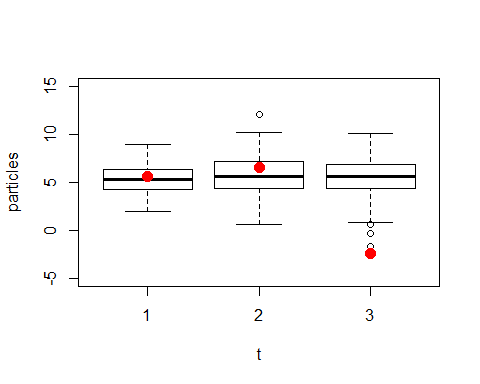
\includegraphics{reproducing_files/figure-latex/unnamed-chunk-1-1.pdf}

\begin{Shaded}
\begin{Highlighting}[]
\CommentTok{# The result is close but not identical to the official seasonally adjusted series.}
\end{Highlighting}
\end{Shaded}

By default, a call to seas also invokes the following automatic
procedures of X-13: * Transformation selection (log / no log);\\
* Detection of trading day and Easter effects;\\
* Outlier detection;\\
* ARIMA model search.\\
In the example above, X-13 opts to perform no pre-transformation, does
not adjust for weekday or Easter effects, detects no outliers and models
the series by a (1 1 1)(0 1 1) seasonal ARIMA (autoregressive integrated
moving average) model. This can be seen from the summary output: There
are no coefficients for Easter or outliers, and the ARIMA specification
and the transformation are shown at the bottom\\
By default, seas calls the \emph{SEATS} adjustment procedure(which
decomposes the ARIMA model).To perform the alternative \emph{X-11}
adjustment procedure, the following option can be used:

\begin{Shaded}
\begin{Highlighting}[]
\KeywordTok{library}\NormalTok{(}\StringTok{"seasonal"}\NormalTok{)}
\KeywordTok{library}\NormalTok{(}\StringTok{"seasonalview"}\NormalTok{)}
\end{Highlighting}
\end{Shaded}

\begin{verbatim}
## Registered S3 method overwritten by 'xts':
##   method     from
##   as.zoo.xts zoo
\end{verbatim}

\begin{verbatim}
## 
## Attaching package: 'seasonalview'
\end{verbatim}

\begin{verbatim}
## The following object is masked from 'package:seasonal':
## 
##     view
\end{verbatim}

\begin{Shaded}
\begin{Highlighting}[]
\NormalTok{eg_seats <-}\StringTok{ }\KeywordTok{seas}\NormalTok{(unemp)}
\NormalTok{eg_x11 <-}\StringTok{ }\KeywordTok{seas}\NormalTok{(unemp, }\DataTypeTok{x11 =} \StringTok{""}\NormalTok{)}
\KeywordTok{plot}\NormalTok{(unemp,}\DataTypeTok{col=}\StringTok{"lightblue"}\NormalTok{,}\DataTypeTok{ylim=}\KeywordTok{c}\NormalTok{(}\DecValTok{5500}\NormalTok{,}\DecValTok{15300}\NormalTok{),}\DataTypeTok{ylab=}\StringTok{""}\NormalTok{)}
\KeywordTok{par}\NormalTok{(}\DataTypeTok{new=}\NormalTok{T)}
\KeywordTok{plot}\NormalTok{(}\KeywordTok{final}\NormalTok{(eg_seats),}\DataTypeTok{col=}\StringTok{"red"}\NormalTok{,}\DataTypeTok{ylim=}\KeywordTok{c}\NormalTok{(}\DecValTok{5500}\NormalTok{,}\DecValTok{15300}\NormalTok{),}\DataTypeTok{ylab=}\StringTok{""}\NormalTok{)}
\KeywordTok{par}\NormalTok{(}\DataTypeTok{new=}\NormalTok{T)}
\KeywordTok{plot}\NormalTok{(}\KeywordTok{final}\NormalTok{(eg_x11),}\DataTypeTok{col=}\StringTok{"blue"}\NormalTok{,}\DataTypeTok{ylim=}\KeywordTok{c}\NormalTok{(}\DecValTok{5500}\NormalTok{,}\DecValTok{15300}\NormalTok{),}\DataTypeTok{ylab=}\StringTok{""}\NormalTok{)}
\end{Highlighting}
\end{Shaded}

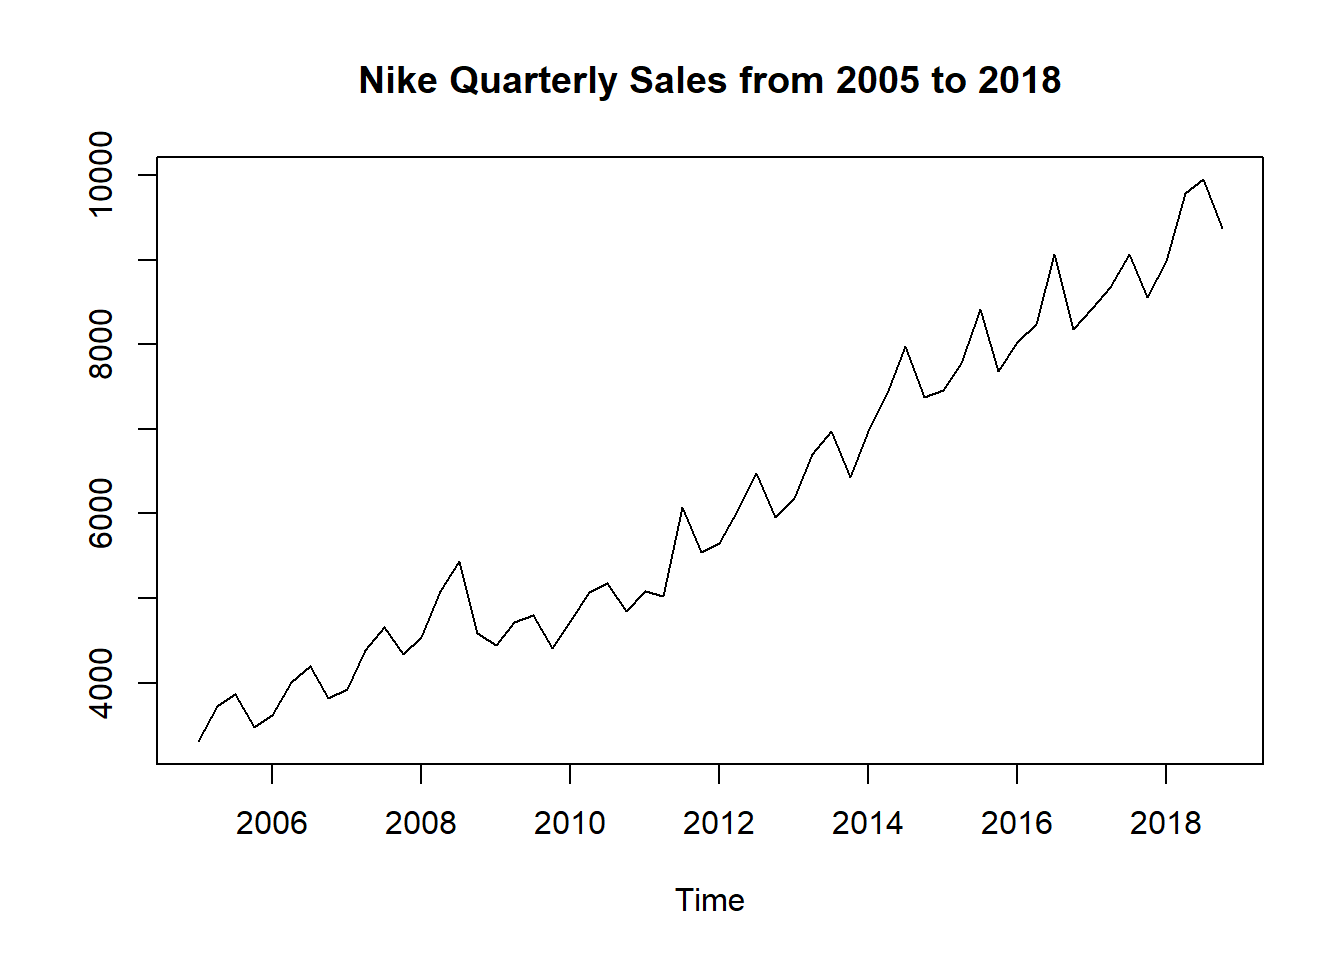
\includegraphics{reproducing_files/figure-latex/unnamed-chunk-2-1.pdf}

\begin{Shaded}
\begin{Highlighting}[]
\KeywordTok{seas}\NormalTok{(}\DataTypeTok{x =}\NormalTok{ unemp,}\DataTypeTok{arima.model =} \StringTok{"(1 1 1)(0 1 1)"}\NormalTok{,}\DataTypeTok{regression.aictest =} \OtherTok{NULL}\NormalTok{,}\DataTypeTok{outlier =} \OtherTok{NULL}\NormalTok{,}\DataTypeTok{transform.function =} \StringTok{"none"}\NormalTok{)}
\end{Highlighting}
\end{Shaded}

\begin{verbatim}
## 
## Call:
## seas(x = unemp, transform.function = "none", regression.aictest = NULL, 
##     outlier = NULL, arima.model = "(1 1 1)(0 1 1)")
## 
## Coefficients:
## AR-Nonseasonal-01  MA-Nonseasonal-01     MA-Seasonal-12  
##            0.9436             0.8254             0.8507
\end{verbatim}

Well, the results here seem to be good.

\hypertarget{lets-try-our-own-data}{%
\subsubsection{Let's try our own data}\label{lets-try-our-own-data}}

\begin{Shaded}
\begin{Highlighting}[]
\KeywordTok{library}\NormalTok{(forecast)}
\end{Highlighting}
\end{Shaded}

\begin{verbatim}
## Registered S3 methods overwritten by 'ggplot2':
##   method         from 
##   [.quosures     rlang
##   c.quosures     rlang
##   print.quosures rlang
\end{verbatim}

\begin{verbatim}
## Registered S3 method overwritten by 'quantmod':
##   method            from
##   as.zoo.data.frame zoo
\end{verbatim}

\begin{verbatim}
## Registered S3 methods overwritten by 'forecast':
##   method             from    
##   fitted.fracdiff    fracdiff
##   residuals.fracdiff fracdiff
\end{verbatim}

\begin{Shaded}
\begin{Highlighting}[]
\KeywordTok{set.seed}\NormalTok{(}\DecValTok{1}\NormalTok{)}
\NormalTok{model <-}\StringTok{ }\KeywordTok{Arima}\NormalTok{(}\KeywordTok{ts}\NormalTok{(}\KeywordTok{rnorm}\NormalTok{(}\DecValTok{24000}\NormalTok{),}\DataTypeTok{freq=}\DecValTok{12}\NormalTok{), }\DataTypeTok{order=}\KeywordTok{c}\NormalTok{(}\DecValTok{0}\NormalTok{,}\DecValTok{1}\NormalTok{,}\DecValTok{1}\NormalTok{), }\DataTypeTok{seasonal=}\KeywordTok{c}\NormalTok{(}\DecValTok{0}\NormalTok{,}\DecValTok{1}\NormalTok{,}\DecValTok{1}\NormalTok{),}\DataTypeTok{fixed=}\KeywordTok{c}\NormalTok{(}\DataTypeTok{theta=}\FloatTok{0.5}\NormalTok{, }\DataTypeTok{Theta=}\FloatTok{0.5}\NormalTok{))}
\NormalTok{data <-}\StringTok{ }\KeywordTok{simulate}\NormalTok{(model,}\DataTypeTok{nsim=}\DecValTok{240}\NormalTok{)}
\KeywordTok{plot}\NormalTok{(data)}
\end{Highlighting}
\end{Shaded}

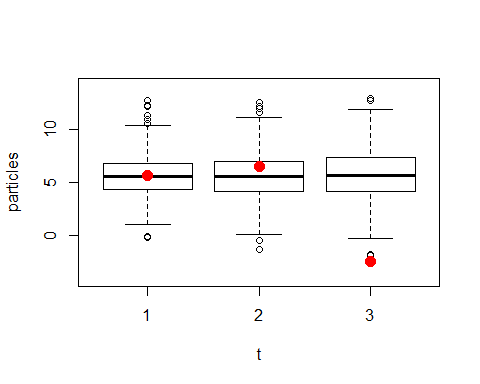
\includegraphics{reproducing_files/figure-latex/unnamed-chunk-3-1.pdf}

\begin{Shaded}
\begin{Highlighting}[]
\NormalTok{m_x11 <-}\StringTok{ }\KeywordTok{seas}\NormalTok{(data, }\DataTypeTok{x11 =} \StringTok{""}\NormalTok{, }\DataTypeTok{regression.aictest =}  \OtherTok{NULL}\NormalTok{)}
\KeywordTok{plot}\NormalTok{(m_x11)}
\end{Highlighting}
\end{Shaded}

\includegraphics{reproducing_files/figure-latex/unnamed-chunk-3-2.pdf}

\begin{Shaded}
\begin{Highlighting}[]
\NormalTok{m_seats <-}\StringTok{ }\KeywordTok{seas}\NormalTok{(data, }\DataTypeTok{regression.aictest =} \OtherTok{NULL}\NormalTok{)}
\end{Highlighting}
\end{Shaded}

\begin{verbatim}
## Model used in SEATS is different: (0 1 1)(0 1 0)
\end{verbatim}

\begin{Shaded}
\begin{Highlighting}[]
\KeywordTok{plot}\NormalTok{(m_seats)}
\end{Highlighting}
\end{Shaded}

\includegraphics{reproducing_files/figure-latex/unnamed-chunk-3-3.pdf}

\begin{Shaded}
\begin{Highlighting}[]
\KeywordTok{plot}\NormalTok{(data,}\DataTypeTok{col=}\StringTok{"green"}\NormalTok{,}\DataTypeTok{ylim=}\KeywordTok{c}\NormalTok{(}\OperatorTok{-}\DecValTok{10}\NormalTok{,}\DecValTok{2000}\NormalTok{),}\DataTypeTok{ylab=}\StringTok{""}\NormalTok{)}
\KeywordTok{par}\NormalTok{(}\DataTypeTok{new=}\NormalTok{T)}
\KeywordTok{plot}\NormalTok{(}\KeywordTok{final}\NormalTok{(m_x11),}\DataTypeTok{col=}\StringTok{"red"}\NormalTok{,}\DataTypeTok{ylim=}\KeywordTok{c}\NormalTok{(}\OperatorTok{-}\DecValTok{10}\NormalTok{,}\DecValTok{2000}\NormalTok{),}\DataTypeTok{ylab=}\StringTok{""}\NormalTok{)}
\KeywordTok{par}\NormalTok{(}\DataTypeTok{new=}\NormalTok{T)}
\KeywordTok{plot}\NormalTok{(}\KeywordTok{final}\NormalTok{(m_seats),}\DataTypeTok{col=}\StringTok{"blue"}\NormalTok{,}\DataTypeTok{ylim=}\KeywordTok{c}\NormalTok{(}\OperatorTok{-}\DecValTok{10}\NormalTok{,}\DecValTok{2000}\NormalTok{),}\DataTypeTok{ylab=}\StringTok{""}\NormalTok{)}
\KeywordTok{legend}\NormalTok{(}\StringTok{"topleft"}\NormalTok{,}\KeywordTok{c}\NormalTok{(}\StringTok{"Data"}\NormalTok{,}\StringTok{"X11"}\NormalTok{,}\StringTok{"SEATS"}\NormalTok{),}\DataTypeTok{col=}\KeywordTok{c}\NormalTok{(}\StringTok{"green"}\NormalTok{,}\StringTok{"red"}\NormalTok{,}\StringTok{"blue"}\NormalTok{),}\DataTypeTok{lty=}\KeywordTok{c}\NormalTok{(}\DecValTok{1}\NormalTok{,}\DecValTok{1}\NormalTok{,}\DecValTok{1}\NormalTok{))}
\end{Highlighting}
\end{Shaded}

\includegraphics{reproducing_files/figure-latex/unnamed-chunk-3-4.pdf}

emmm, I am confused that why the result from the \emph{SEATS} is
different from that out of \emph{X-11}. The model from X-11 is
\((0,1,1)(0,1,1)_{12}\) but SEATS gives me \((0,1,1)(0,1,0)_{12}\). The
former one is right and the corresponding estimation of
\(\theta, \Theta\) is also close.

\hypertarget{seats}{%
\section{SEATS}\label{seats}}

See above.

\hypertarget{state-space-model}{%
\section{State Space Model}\label{state-space-model}}

I just spent a whole day working on the state space model, trying to
figure out the steps in this process. To be honest, I was not very, like
80\%, clear about bootstrap particle filter, although I spent much time
on it during last term. But I have to admit the effort I paid before is
worthy, otherwise I can't come up with the following code within one
day. The resource is mainly from \textbf{BOOK Monte Carlo Statistical
Methods} and the
\href{https://onlinelibrary.wiley.com/doi/abs/10.1111/1467-842X.00104}{lecture}.

\begin{Shaded}
\begin{Highlighting}[]
\KeywordTok{library}\NormalTok{(forecast)}
\KeywordTok{set.seed}\NormalTok{(}\DecValTok{1}\NormalTok{)}
\NormalTok{model <-}\StringTok{ }\KeywordTok{Arima}\NormalTok{(}\KeywordTok{ts}\NormalTok{(}\KeywordTok{rnorm}\NormalTok{(}\DecValTok{24000}\NormalTok{),}\DataTypeTok{freq=}\DecValTok{12}\NormalTok{), }\DataTypeTok{order=}\KeywordTok{c}\NormalTok{(}\DecValTok{0}\NormalTok{,}\DecValTok{1}\NormalTok{,}\DecValTok{1}\NormalTok{), }\DataTypeTok{seasonal=}\KeywordTok{c}\NormalTok{(}\DecValTok{0}\NormalTok{,}\DecValTok{1}\NormalTok{,}\DecValTok{1}\NormalTok{),}\DataTypeTok{fixed=}\KeywordTok{c}\NormalTok{(}\DataTypeTok{theta=}\FloatTok{0.5}\NormalTok{, }\DataTypeTok{Theta=}\FloatTok{0.5}\NormalTok{))}
\NormalTok{data <-}\StringTok{ }\KeywordTok{simulate}\NormalTok{(model,}\DataTypeTok{nsim=}\DecValTok{240}\NormalTok{)}
\CommentTok{# let's try SIS(Sequential Importance Sampling) at first}
\end{Highlighting}
\end{Shaded}


\end{document}
